\documentclass[a4paper]{ctexart}
\usepackage{geometry}
\usepackage{multicol}
\usepackage{pstricks}
\usepackage{graphics,graphicx}
\usepackage{pst-plot}
\usepackage{color}
\usepackage{amsmath}
\geometry{left=2cm,right=2cm,top=2.5cm,bottom=2.5cm}

\setCJKmainfont[BoldFont={SimHei},ItalicFont={KaiTi}]
  {FangSong}

\author{Chunwei Yan}
\title{全书解答5}
\begin{document}
    \maketitle
%---content here----
\begin{multicols}{2}

\section{P136例9}
\subsection{知识点}
知识点不熟悉的话,那部分的内容回顾一下。
\begin{enumerate}
    \item 二元函数$f(x,y)$在某一点处的偏导数的求法见:全书P129\quad 三、二元函数的偏导数与全微分)
    \item 用定义法证明二元函数可微(见:全书P134\quad 三、讨论函数的可微性)
\end{enumerate}

\subsection{解答}
\subsubsection{用定义求偏导}
\par
首先,第一部分是偏导数的求法
\par 这里利用了偏导的定义法来求解,比如求解$f'_x(x,y)$
\begin{enumerate}
    \item 控制和排除无关变量,对$x$求偏导,我们暂时对$y$不感兴趣,因为在点$(0,0)$处,直接将$y=0$,此时二元函数实际上变成了一个一元函数$z=f(x,0)$
    \item 利用极限的定义,求解$f'_x(0,0)$,
    $$
        f'(0,0) =\lim_{\Delta x\rightarrow 0}{ \frac{f(0+\Delta x, 0) - f(0,0)}
                        {\Delta x - 0}}
    $$
\end{enumerate}
\par
\textbf{注意偏导和全微分的区别,偏导数是一次只对一个或者几个自变量求导(如$f'_x(x_0, y_0)$,而全微分是同时对所有的自变量求导}

\subsubsection{用定义判断是否可微}
参照P134的方法,思路就是判断
$$
\Delta z = [f(x_0+\Delta x, y_0 + \Delta y) - f(x_0, y_0)]
$$
$$
\lim_{\Delta x\rightarrow 0, \Delta y\rightarrow 0}
$$
$$
\frac{
        \Delta z 
        -
        [f'_x(x_0, y_0)\Delta x + f'x(x_0, y_0)\Delta y]
    }
    {\sqrt{(\Delta x)^2 + (\Delta y)^2}}
$$
是否为0, 如果为0则可微,否则不可微。

\subsection{总结}
\par 这道题很好,多元函数这部分题型很固定,好好记忆一下。 
\par 是否可微的判断,有两种方法
\begin{enumerate}
    \item 利用定义证明,也就是本题的方法
    \item 如果满足其每一个偏导存在且连续,则可微
\end{enumerate}


\section{P136例10}
\subsection{知识点}
\begin{enumerate}
    \item 用定义求偏导
    \item 极限
    \item 用定义判断是否可微
\end{enumerate}

\subsection{问题一,用定义求偏导}
\par 按照定义求偏导,综合利用极限
$$
\lim_{\Delta x\rightarrow 0} 
{
    \frac{
        f(\Delta x, 0) - f(0,0)
    }
    {\Delta x}
}
=
\lim_{\Delta x}
{
    \frac{
        \left| \Delta x \right| \rho(\Delta x,0)
    }
    {\Delta x}
}
$$
\par
不要被这里的$\Delta x$吓住了,一视同仁,这个就是最简单的极限求解,$\Delta x$就是一个普通的变量。
\par
$
\frac{
    \left| \Delta x \right| 
}
{\Delta x}
$
\par
就是一个求符号的运算,会分为$+,-$两种情况。
\par
相应也就得到
$$
= 
\begin{cases}
    \begin{array}{ll}
    \rho(0,0)   &   \Delta x \rightarrow 0+\\
    -\rho(0,0)  &   \Delta x \rightarrow 0-
    \end{array}
\end{cases}
$$
\par
由一元函数的极限(二元函数的偏导降维为一维)的定义可以得到,极限存在必须左右极限相等,也就是$\rho(0,0) = -\rho(0,0) = 0$
\par
由于题目中已经点出,$\rho(x,y)$在点$(0,0)$的邻域内连续,因此$\lim_{\Delta x\rightarrow 0}{\rho(\Delta x,0)} = \rho(0,0)$


\subsection{问题二,用定义判断可微}
\par 判断可微与否的方法有两种
\begin{enumerate}
    \item 利用定义判断
    \item 利用各偏导存在且连续
\end{enumerate}
\par 但是此处无法判断偏导连续,因此用定义法。 用定义法的话,一般就常规地算出来就可以了。 因为形式有点复杂,所有没有什么太难的必要。 所以,套路很明显。
\par \textbf{\textcolor{red} {注意$\Delta x$也是常规的变量,用极限的方法常规对待就可以了}}

\section{P139例9}
答案应该是对的吧
\subsection{知识点}
\par 求偏导的方法,主要分为两个步骤
\begin{enumerate}
    \item 控制无关变量,将不需要偏导的变量用常数替代,或者视为常数
    \item 对剩下的一元函数求导
\end{enumerate}
\par 函数微分的表示见P130\quad 4.可微的必要条件
$$
dz = 
\frac{\partial z}
{\partial x}dx
+
\frac{\partial z}
{\partial y}dy
$$

\subsection{解答}

$$
df(1,1,1) = f'_x(x,1,1)dx + f'_y(1,y,1)dy + f'_z(1,1,z)dz
$$
其中$f'_x(x,1,1)$是$f(x,y,z)$在点$(1,1,1)$处对$x$求偏导形成的,对$x$求导,控制无关变量$y,z$,均分别用1替代。
\par 你可以再做一下.

\section{P146例28}
这个题目比较活,你可以跳过去


\section{P149例33}
这个是典型题,好好把握

\subsection{知识点}
复合求偏导
\begin{center}
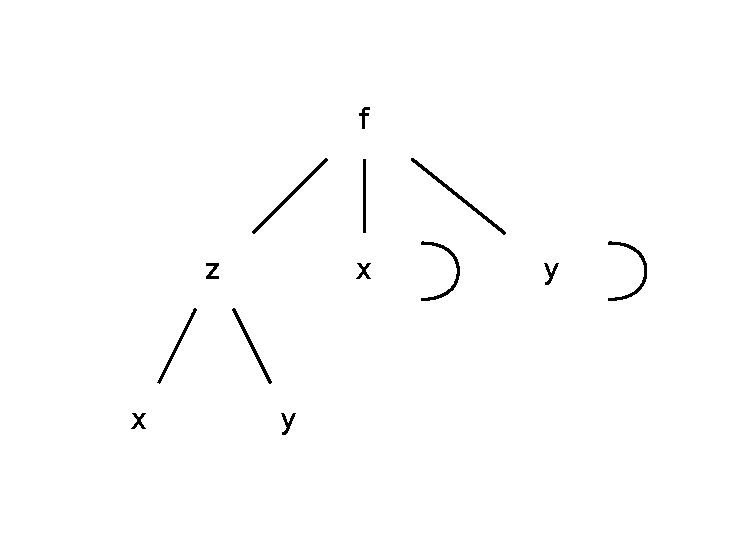
\includegraphics[height=5cm]{split.pdf}
\end{center}
$$
\frac{ \partial z } {\partial x}
 = 
 f' * (1 + 
    \frac{\partial z}
    { \partial x}
    )
$$
\par
左右都有
$ \frac{ \partial z } {\partial x} $
,提取出来,可以计算到

\begin{equation}
\frac{
    \partial z
}
{
    \partial x
}
 = 
 \frac{f'} {1 - f'}
\end{equation}
\par 其中$f'$是$f'(x+y+z)$的简写
\par 下面的挑战是求
$
\frac{{\partial z}^2}
{{\partial x}^2}
$
\begin{equation}
\frac{{\partial z}^2}
{{\partial x}^2}
=
\frac{
    \partial
    \frac{
        \partial z
    }
    {
        \partial x
    }
}
{\partial x}
=
\frac{
     \partial \frac{f'} {1 - f'}
}
{
    \partial x
}
\end{equation}
\par 平常心,不要被形式迷惑。下面就是简单的求导
\par 设想f是关于x的函数,对x求偏导
$$
\frac{
     \partial \frac{f'} {1 - f'}
}
{
    \partial x
}
=
\frac{
     \partial (-1 + \frac{1} {1 - f'})
}
{
    \partial x
}
$$
$$
= 
\frac{
    \partial \frac{1}{1-f'}
}
{\partial x}
$$
把$f$看作$x$的函数,进行分式的求导就可以得到最后的结果
$$
=
- \frac{1}{(1-f')^2}
\frac{\partial f'}
{\partial x}
$$
其中
$$
\frac{\partial f'}
{\partial x}
=
\frac{\partial f'(x+y+z)}
{\partial x}
= 
f{''}
* 
\frac{\partial (x+y+z)}
{\partial x}
=
f{''}
* 
1 + 
\frac{\partial +z}
{\partial x}
$$
根据公式(1)可以将$\frac{\partial z}{\partial x}$用$f'$表示,最终结果就得出来了。

\subsection{衍生}
$z''_{xy}$表示$z$分别对$x,y$进行偏导
$$
z''_{xy}
=
\frac{\partial \partial z}
{\partial x\partial y}
=
\frac{\partial \frac{\partial z}{\partial x}}
{\partial y}
=
\frac{\partial \frac{\partial z}{\partial y}}
{\partial x}
$$
一步一步进行求导就可以了。
题目中$\frac{\partial y}{\partial x}=0$,因为题目中没有交代$y$可以被$x$表示。

\section{P150例35}
\subsection{知识点}
\par 这里需要知道$f(x,y)$, 
\begin{itemize}
    \item $f'_1$表示对第一个自变量求偏导, 也就是$f'_x$
    \item $f'_2$表示对第二个自变量求偏导, 也就是$f'_y$
    \item $f''_{12}$表示先对第一个自变量求偏导,然后对第二个自变量求偏导,也就是$f''_{xy}$
\end{itemize}

\subsection{解答}
\begin{equation}
- \frac{
    (f''_{11} + f''_{12}\frac{dy}{dx}f'_2   - (f''_{21} + f''_{22}\frac{dy}{dx})f'_1 
}
    {
        {f'_2}^2
}
\end{equation}
\par 将第2行$\frac{dy}{dx} = - \frac{f'_1}{f'_2}$代入其中,分式上下同乘$f'_2$就得到最后结果了。


\section{P155 例43}
\subsection{知识点}
\par 求多元函数的最值,详见全书P154
\par 总之就是讨论其特殊点,包括
\begin{enumerate}
    \item 极值点
    \item 驻点(一阶导数为0的点)
    \item 边界上的点(利用拉格朗日法求解条件极值)
\end{enumerate}

\subsubsection{条件极值}
\par 条件极值方面参照全书P151 \quad 条件极值
\begin{enumerate}
\item 要求函数 $f(x,y,z)$ 在条件 $\varphi(x,y,z)=0$下的极值
\par 就构造拉格朗日函数,用参数$\lambda$将函数和条件结合在一起
$$
F(x,y,z,\lambda) = f(x,y,z) + \lambda \varphi(x,y,z)
$$
\par 相应地,有多少个条件,就设几个参数
\par 比如,如果有两个条件的时候:
\item 要求函数 $f(x,y,z)$ 在条件 $\varphi(x,y,z)=0, \phi(x,y,z)$下的极值
$$
F(x,y,z,\lambda,\mu) = f(x,y,z) + \lambda \varphi(x,y,z) + \mu \phi(x,y,z)
$$
\textbf{\textcolor{red}{条件极值是基础题型,固定题型,记住就行。很常考。好好看看.}}
\end{enumerate}


\subsection{解答}
\subsection{第一部分,多元函数的极值}
\par 详见P151\quad 对这个要有印象
$$
\begin{array}{ll}
AC - B^2 > 0  & small\\
AC - B^2 < 0  & big\\
AC - B^2 = 0  & unknown
\end{array}
$$
\par 如果有点不熟悉要好好看看,每天都看,都练,肯定能够熟练的

\subsection{条件极值}
\par 上面一部分对区域D内部的点求极值和驻点
\par 下面需要去讨论边界上的最大值。 考虑函数在边界上的最值,无非也就是一种条件极值。
\par 函数是$z = x^2 + y^2 -12 x + 16y$,条件只有一个,是$x^2 + y^2 = 25$,于是设立一个参数$\lambda$,统一起来构造拉格朗日函数
$$
F(x,y,\lambda) = \cdots
$$
\par 这个就是解答里面的式子

\section{P158 例46}
\subsection{知识点}
\par 这里有一个公式,你也许不知道,需要记忆一下
\par 任意一个三角形的面积$S$和周长$C$之间有一定的关系
\par 假设$p = \frac{C}{2}$,就会有
$$
S = \sqrt{p(p-x)(p-y)(p-z)}
$$

\subsection{解答}
\par 第2行会得到$h$和$\sqrt{p(p-x)(p-y)(p-z)}$的一个关系,替换到体积的公式里面,就会得到
$$
V = \frac{4}{3}\pi p 
        \frac{(p-x)(p-y)(p-z)}{y}
$$
\par 这里会有一个技巧,因为连乘的$x,y,z$无法求导,一般有连乘或者幂函数的时候,采用求对数的方法将乘积变成求和
\par 再接下来就是常规的条件极值了

\subsection{总结}
\par 可以看到,这类综合题,尽管步骤比较多,但是也就是一些基础的知识点和题型的组合,如果自己的知识点和题型都比较熟悉的话,肯定能够按部就班做出来的。
\par 所以,重点还是知识点和基础题型。
\par 题目中发现有不懂的点,是好事,现在还额可以好好练好。

\section{P158 例47}
\subsection{知识点}
\begin{pspicture}(-4,-3)(4,4)
%\psgrid[subgriddiv=1,griddots=10,gridlabels=7pt](-3,-3)(3,3)
\psaxes{->}(0,0)(-3.5,-2.7)(3.5,2.7)
\psellipse(0,0)(2,1)
\rput[lb](2, 0){A}
\rput[rb](-2, 0){$A'$}
\rput[lb](0,0){O}
\rput[lb](0,1){B}
\end{pspicture}

\begin{itemize}
    \item 其中线段OA就是长半轴(AA'是长轴),可以看到A是离椭圆中心最远的一点
    \item 线段OB就是短半轴,可以看到B是离椭圆中心最近的一点
\end{itemize}
\par 题目就是根据这个,从离中心距离的最值来得到长半轴和短半轴

\subsection{解答}
\par P159上面的解答得到$x^2 + y^2 = -\lambda$
\par 然后下面得到$\lambda = -3 \pm 2\sqrt{2}$,这两个值代表了椭圆上点$(z,y)$离中心的最值,于是,更具上面的分析,得到长半轴$a = \sqrt{3+2\sqrt{2}} = \sqrt{1 + 2\sqrt{2} + \sqrt{2}^2} = \sqrt{(1+\sqrt{2})^2} = 1+\sqrt{2}$
\par 相应短半轴$b = \sqrt{1 - 2\sqrt{2} + \sqrt{2}^2} = \sqrt{(\sqrt{2} - 1)^2} = \sqrt{2} - 1$

\section{P163 例50}
\subsection{知识点}
\par 判断其关于$y=x$,只需要将式子里面的所有$x$和$y$互换,如果得到的值相同,则其对称

\subsection{解答}
\par 方法二,采用非常巧妙的排除法
\par 假设$f(x)=1$,也就是说$f(x)$是一个常值函数,永远等于1,于是积分就一目了然了
$$
\cdots = \iint_{D}{(a+b)}d\sigma = (a+b)S_D = \frac{(a+b)}{2}\pi
$$
\par 一下子就得到结果了
\par 其中$\iint_{D}d\sigma$就是此区域的面积

\subsection{总结}
\par 二元函数积分方面,要充分利用对称等技巧,会极大地降低计算复杂度。 毕竟,真题里面不会单纯让死算的。











%------ end content --------------
\end{multicols}
\end{document}
